\documentclass[11pt]{article}
\usepackage[margin=1in]{geometry}
\usepackage{amsmath, amssymb, amsthm, enumerate}
\usepackage{graphicx,url, hyperref,framed, esint, color, tikz}
\usepackage{listings}

\usepackage{fancyhdr}

\pagestyle{fancy}
\renewcommand{\sectionmark}[1]{\markboth{#1}{}} % set the \leftmark

\fancyhf{}
\fancyhead[L]{\leftmark} % 1. sectionname
\fancyfoot[C]{\thepage}
\fancypagestyle{plain}{%
  \fancyhf{}%
  \renewcommand{\headrulewidth}{0pt}%
}

\setcounter{secnumdepth}{-2}


\lstset{language=C,
                basicstyle=\ttfamily,
                keywordstyle=\color{blue}\ttfamily,
                stringstyle=\color{red}\ttfamily,
                commentstyle=\color{purple}\ttfamily,
                morecomment=[l][\color{magenta}]{\#},
                showstringspaces=false
}

\begin{document}
\thispagestyle{empty}
\begin{flushright}
Alex Rich and Aaron Rosen\\
Engineering 155 \\ 
Final Project Status Report\\
November 23, 2015
\end{flushright}
\section{Project Status Report: A Robot Controlled Over The Internet}

The team has made progress on a robotic vehicle that receives user input from a website and executes the commands. The website is hosted by an E155 Raspberry Pi2 Apache2 server, and contains a visual grid interface.  The grid represents different locations on the ground with respect to the vehicle.  To send the vehicle to the desired location, the user clicks on the corresponding point on the grid, which inputs commands into a buffer to be sent to the vehicle.  The Pi will parse the commands and send them wirelessly using a Belkin FT8001 Bluetooth dongle to a BlueSMiRF located on the vehicle.  The vehicle's controller (the E155 $\mu$Mudd board) reads these commands and executes them. An overview of this system is shown in Figure \ref{fig:sys}. Below we discuss the current status for each part (website, Pi, FPGA, vehicle, new hardware) in detail.

\subsection{Website}
The website currently contains a visual user interface that contains instructions for use, a grid on which to input locations for the robot to maneuver to, a list of the locations currently buffered for sending, and an option to clear the buffer. The code for the website is shown in Appendix A. The website was built using HTML, Javascript, and Bootstrap CSS. 

The Pi hosts the website. Upon clicking in a grid space, the page's javascript will eventually calculate the left and right tread speeds and duration of movement required to get the tank to move from its original position to the new position. Currently, it creates a random command to be sent to the FPGA. Next, the javascript makes an HTTP GET request to the inputChars resource of the Pi. When the request is completed, the page updates, either submitting the next command in the buffer or waiting for another input from the user.


\subsection{Raspberry Pi 2}

After receiving a GET request, the common gateway interface (CGI) reads the input parameters and calls a Python script. The Python script utilizes the \verb.bluetooth. module to allow sending data using the bluetooth dongle. Since the robot has a constant bluetooth device address, this address is hard coded into the Python script. When called, the python script sends the commands, one at a time, to the robot. Currently, the system sleeps for an amount of time to theoretically give the vehicle enough time to move. However, in the future, the Pi will wait for acknowledgement from the FPGA. The code on the Pi is shown in Appendix B. Figure \ref{fig:piroutines} show the flow of data and control through the Pi.

\begin{figure}
\begin{center}
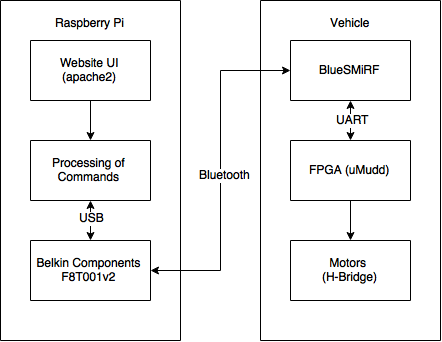
\includegraphics[width=0.7\textwidth]{E155System}
\end{center}
\caption{An overview of the system. The system is comprised of two major subsystems: the Raspberry Pi 2 controller and the vehicle, which is controlled by the $\mu$Mudd board.}
\label{fig:sys}
\end{figure}

\begin{figure}
\begin{center}
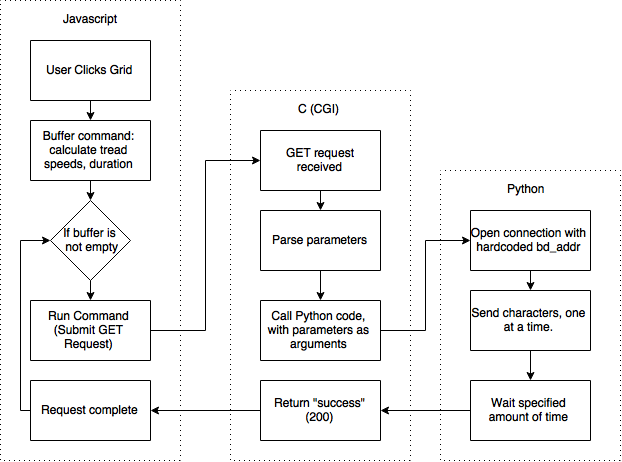
\includegraphics[width=0.8\textwidth]{PiRoutines}
\end{center}
\caption{The flow of control and data through the Pi.}
\label{fig:piroutines}
\end{figure}

\subsection{FPGA}
The FPGA reads data from a BlueSMiRF using UART hardware coded in SystemVerilog and then processes and executes the command.  It is constructed as a controller-datapath pair with three main submodules - receiveMSG, executeCommand, and sendAck.  The SystemVerilog code running on the FPGA is shown in Appendix C. The FPGA and BlueSMiRF are the only two electrical components on the breadboard. The schematic is shown in figure \ref{fig:breadboard}

The clock used to interface with the BlueSMiRF is implemented using a PLL that oversamples the 112.5 Kbaud frequency by a factor of 8.  This oversampler determines if there is an incoming message.  The actual sampling of the BlueSMiRF's TX line is accomplished using a frequency divider that allows for sampling at the correct rate.  The divider's phase can be controlled in order to ensure that the sampling of the line is as close to the center of the transmission's clock as possible.  As there are three characters in each command, the code holds the system in the receiveMSG state until all three characters have been loaded.

The FPGA executes the command received by controlling the two motors via the H-Bridges on the $\mu$Mudd board. Each command consists of a PWM setting for each motor and a duration for which the motors should be running.  A counter is used to create a reference clock for PWM; the power levels are referenced against this counter to determine the correct duty cycle.  To prevent the vehicle from running indefinitely, the timer stops incrementing when the requested duration is reached, and a signal is output that is used to cut power to the motors.  Each LSb of the duration char corresponds to roughly one-tenth of a second duration.

Once the requested duration has been reached and power to the motors cut, the FPGA transmits the character `A' back to the BlueSMiRF as an ACK code.  After this ACK has been sent, the FPGA will cycle around to the receiveMSG state again.

At this time, the $\mu$Mudd board interfaces with the BlueSMiRF.  All parts of the code have been written; however there are still critical bugs in the code to be worked out.  The receiveMSG and controller modules have been independently verified in ModelSim.  The other two main submodules will be independently verified shortly, and then the whole system will be tested together.

Figure \ref{fig:fpga} shows a high level block diagram of the FPGA, with more detailed diagrams in Appendix D.

\begin{figure}
\begin{center}
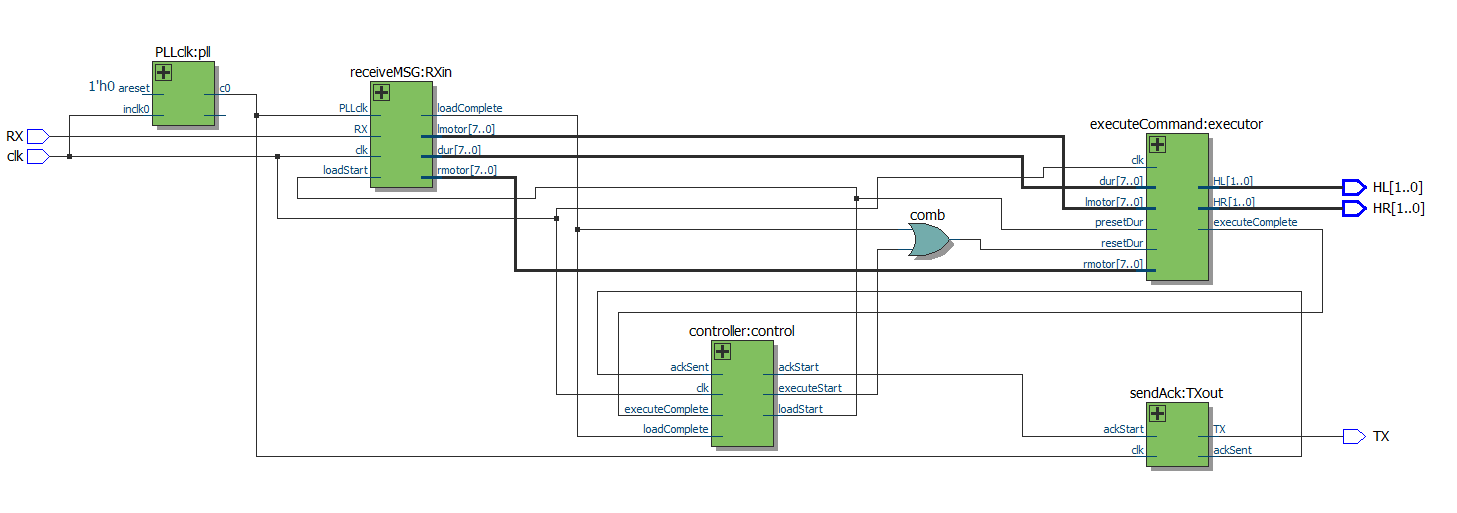
\includegraphics[width=\textwidth]{systemOverview}
\end{center}
\caption{The schematic of the hardware in the FPGA. More detailed diagrams are shown in Appendix D.}
\label{fig:fpga}
\end{figure}

\subsection{Vehicle}
All of the parts for the vehicle have been ordered and received. The vehicle has yet to be assembled, as there will be no machining or fabrication involved at this point.

\begin{figure}
\begin{center}
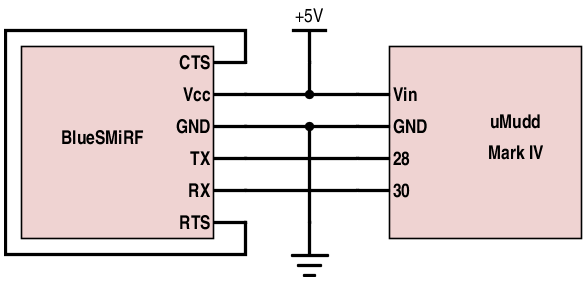
\includegraphics[width=0.7\textwidth]{breadboard}
\end{center}
\caption{The schematic of the circuit on the breadboard. In simple applications, the CTS and RTS pins of the BlueSMiRF are connected together, and the only pins that are connected to the FPGA are TX and RX.}
\label{fig:breadboard}
\end{figure}



\section{Appendix A: Website}
\subsection{Code}

\lstinputlisting[language=html]{../pi/final.html}

\subsection{Result}

Figure \ref{fig:page} shows the website user interface that appears when accessing the raspberry pi. The grid is clickable, and the buffer of commands is listed on the right side of the page. A user can also submit a direct command using the form on the right.

\begin{figure}[!h]
\begin{center}
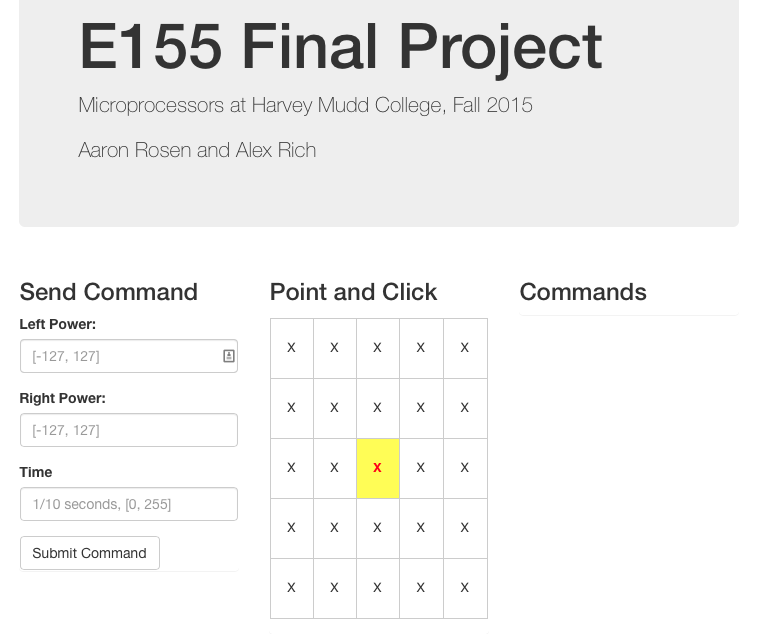
\includegraphics[width=0.9\textwidth]{page}
\end{center}
\caption{The website displayed to a user controlling the robot.}
\label{fig:page}
\end{figure}

\section{Appendix B: Raspberry Pi2 Code}
\subsection{CGI Code}
\lstinputlisting[language=C]{../pi/inputChars.c}
\subsection{Python Code}
\lstinputlisting[language=Python]{../pi/sendData.py}

\section{Appendix C: SystemVerilog Code on FPGA}
\lstinputlisting[language=Verilog]{VehicleControl2.sv}

\section{Appendix D: FPGA Diagrams}

\begin{center}
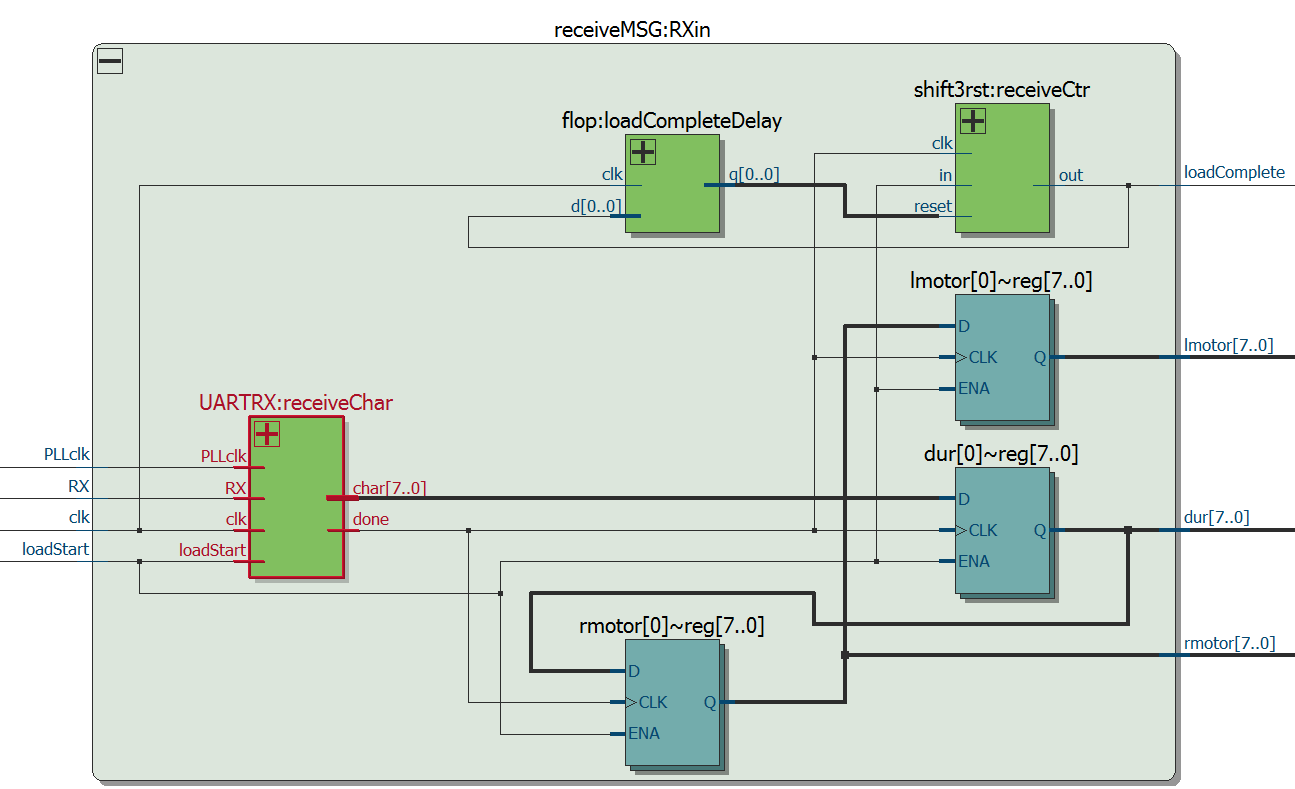
\includegraphics[width=\textwidth]{receiveMSG}
\end{center}

\begin{center}
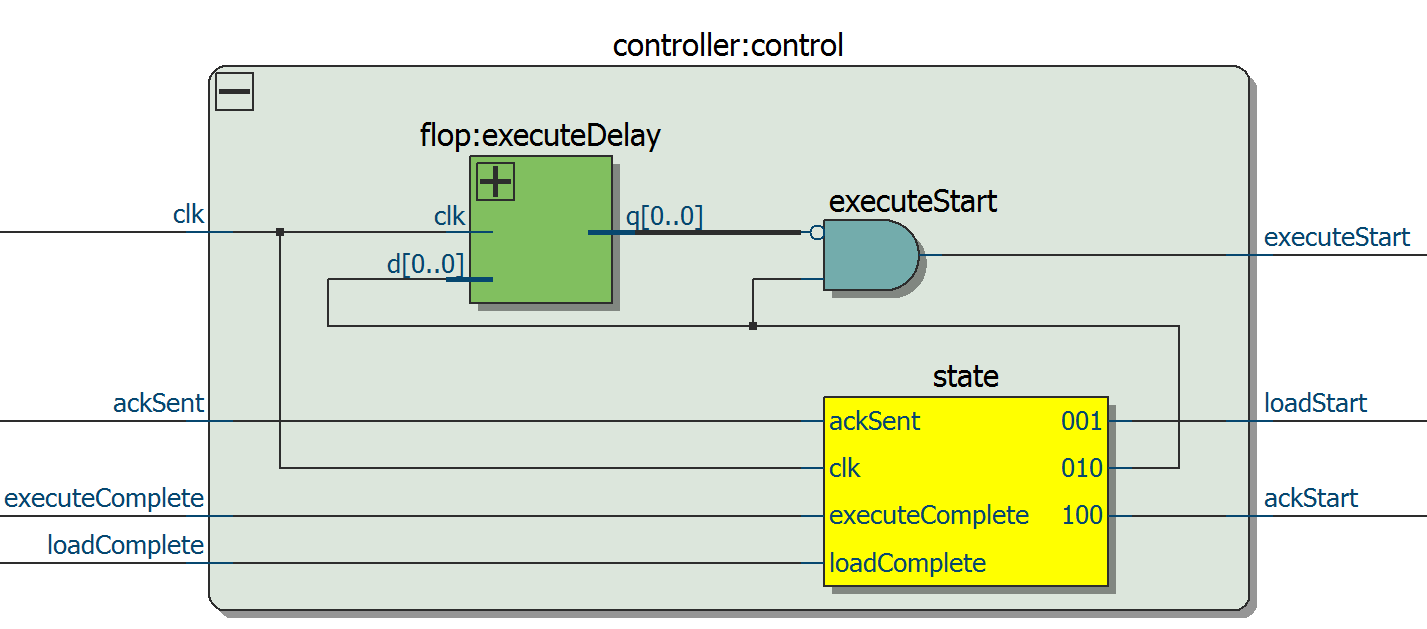
\includegraphics[width=\textwidth]{controller}
\end{center}

\begin{center}
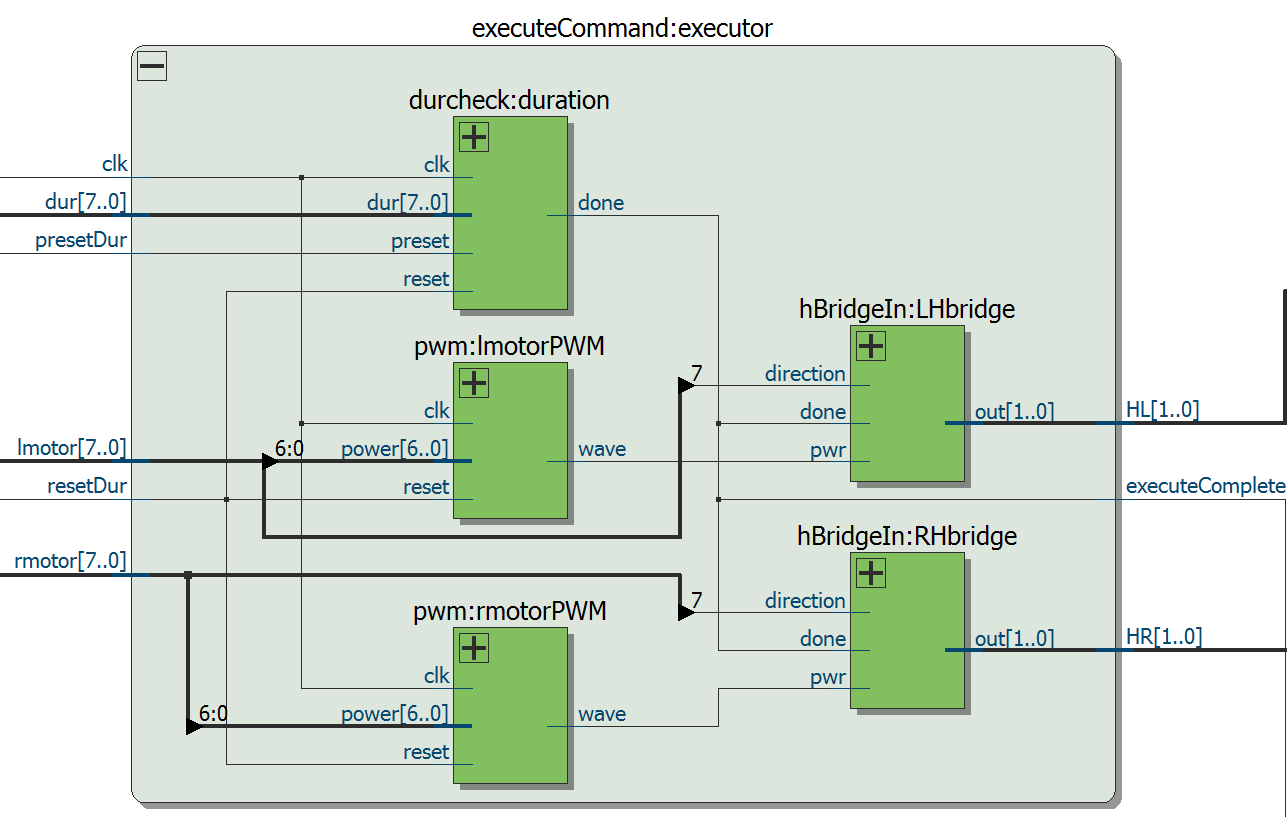
\includegraphics[width=\textwidth]{executeCommand}
\end{center}

\begin{center}
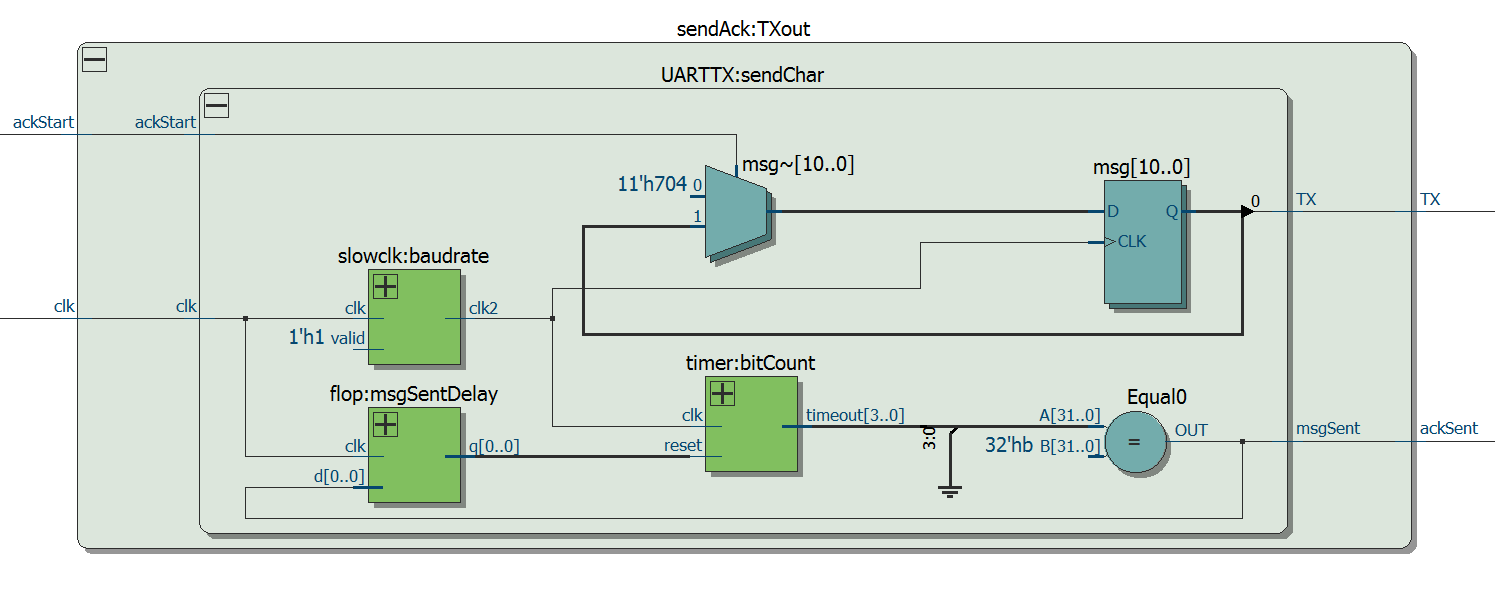
\includegraphics[width=\textwidth]{sendAck}
\end{center}

\section{Appendix E: Bill of Materials}
This is the bill of materials for the project.

\centering
\begin{tabular}{|l|l|l|l|}
\hline
\multicolumn{1}{|c|}{\textbf{Item}} & \multicolumn{1}{c|}{\textbf{Description}}               	& \multicolumn{1}{c|}{\textbf{Source}} & \multicolumn{1}{c|}{\textbf{Cost}} \\ \hline
Tracked Vehicle 			&										&							&	\\
			Chassis Kit	& Chassis for the tank, includes treads and frame.    	& Amazon 					& 15.39                          	\\ \hline
Tamiya 70168				& Gives tank flexibility to turn by controlling each     	& 							& \\
Double Gearbox			& tread independently.						& Amazon		               			& 11.99                             	\\ \hline
$\mu$Mudd Board                	& Controls the vehicle.                                                & E155                                 		& 0.00                               	\\ \hline
			                      	& Provides website interface and sends commands 	&							&\\
Raspberry Pi 2			    	& to vehicle.             							& E155                                 		& 0.00                               	\\ \hline
                        				& Wirelessly communicate via Bluetooth between  	&							&\\
BlueSMiRF				& Pi and $\mu$Mudd board.		 			& E155                                		& 0.00                               	\\ \hline
Belkin Components FT8001	& Send bluetooth data from Pi.					& E155                                		& 0.00                               	\\ \hline
2X TrustFire 14500			& Li Ion battery, 3.7 V 						& Aaron Rosen					& 0.00				\\ \hline
\end{tabular}

\end{document}


























